\chapter{モデルベースシステムズエンジニアリング}
%高井さん
\label{chap4}

\section{システムズエンジニアリングの基礎}

\subsection{システムズエンジニアリングとは}
システムエンジニアリング(systems engineering)は、分野に依存せず「シス
  テム」を構築したり発展させたりするための知見をまとめたものです。従来
は、製品やサービスの領域毎に、開発プロセスは発展し、その中での最適化が
行われてきました。しかし、多くのシステムが大規模化、複雑化するなかで、
領域毎に発展してきた方法論では、必要な納期を満たせなかったり品質を保証
することが難しくなってきました。一方で、そのような課題は、製品やサービ
スに依存しない現象として説明したり、さらにはその解決アプローチについて
も、一般化して検討できるかもしれない、と気付いた人たちがいました。その
ような知見をまとめたものがシステムズエンジニアリングであり、実際多くの
現場でその効果が確かめられたため、国際標準化なども含めて普及が進んでい
ます。

システムズエンジニアリングは例えば次のように定義
されます(\lbrack JIS X 0170\rbrack)。
\begin{quote}
  利害関係者のニーズ、期待及び制約の集合を、解決するソリューションへ変
  換するため、及びソリューションが用いられる全期間を通じて、それを支援
  するために要求される,技術上及び管理上の作業の全体を統括するような、
  複数の専門分野を横断した取組方法。
\end{quote}
一つ一つ見ていきましょう。
\begin{quote}
  利害関係者のニーズ、期待及び制約の集合を、解決するソリューションへ変
  換する
\end{quote}
はじめに、システムズエンジニアリングの目的が言及されています。ここでは、
利害関係者がそれぞれのニーズを持っており、さらに明示化されていない期待
や、実現に対して課せられる制約を考慮した上で、ソリューションを得ること
であることが分かります。このソリューションで中心的な役割を果たすのが典
型的にはシステムとなります。
\begin{quote}
  及びソリューションが用いられる全期間を通じて、
\end{quote}
「全期間」が対象になります。例えば、ニーズを集めるところや企画段階や、
ソリューションの運用が終わったあとの破棄などの期間も対象となります。
\begin{quote}
  それを支援するために要求される,技術上及び管理上の作業の全体を統括す
  るような、
\end{quote}
ソリューションを支援するための、管理上必要となる作業までが対象であるこ
とが分かります。例えば、ソリューションの運用に人系が必要であれば、人的
リソースの管理なども対象に含まれます。
\begin{quote}
  複数の専門分野を横断した取組方法。
\end{quote}
例えば、機械分野や建築分野、電気分野などは、それぞれの分野に特化した方
法論があるかもしれませんが、システムズエンジニアリングで目指すのは、複
数の専門分野の知見が必要となるようなソリューションに対して分野横断的に
適用可能な取組方法であることが分かります。
\subsection{システムエンジニアリングの知見}

システムエンジニアリングにはさまざまな知見が含まれますが、ここでは次の三つを紹介します:

\begin{enumerate}
    \item システムに関する概念の定義
    \item システムの開発や運用においてありうる活動の定義
    \item システムを記述するために必要な観点の提供
\end{enumerate}

\subsection{システムに関する概念の定義}
前述の通り、システムが大規模化、複雑化すると、複数の製品やサービス領域
を組み合わせることが一般的になり、これまで交流のなかった技術者も共同作
業をしなければなりません。そのようなときに共通言語を与えるのも、システ
ムズエンジニアリングの役割です。また、大規模かつ複雑なシステムは、その
開発や運用プロセスも複雑になり、その計画を立てたり、人員を割り当てる際
にも活動に関する共通言語が必要になります。それら開発や運用に係わる活動
に関する概念も、提供する共通概念の重要な部分です。

例えば、ジェットエンジンを開発するときには、巨大な試験施設が必要になり
ます。そのような施設もシステムであり、それ自体がライフサイクルを持ち、
試験対象であるジェットエンジンのライフサイクルも意識しながら施設を開発
し、運用する必要があります。開発や運用対象のシステムを対象システム
(system-of-interest)と呼ぶのに対し、開発時に連携が必要となるシステム
をイネーブリングシステム(enabling system)と呼びます
(\ref{figure:ch4-1})。
\begin{figure}
    \begin{center}
    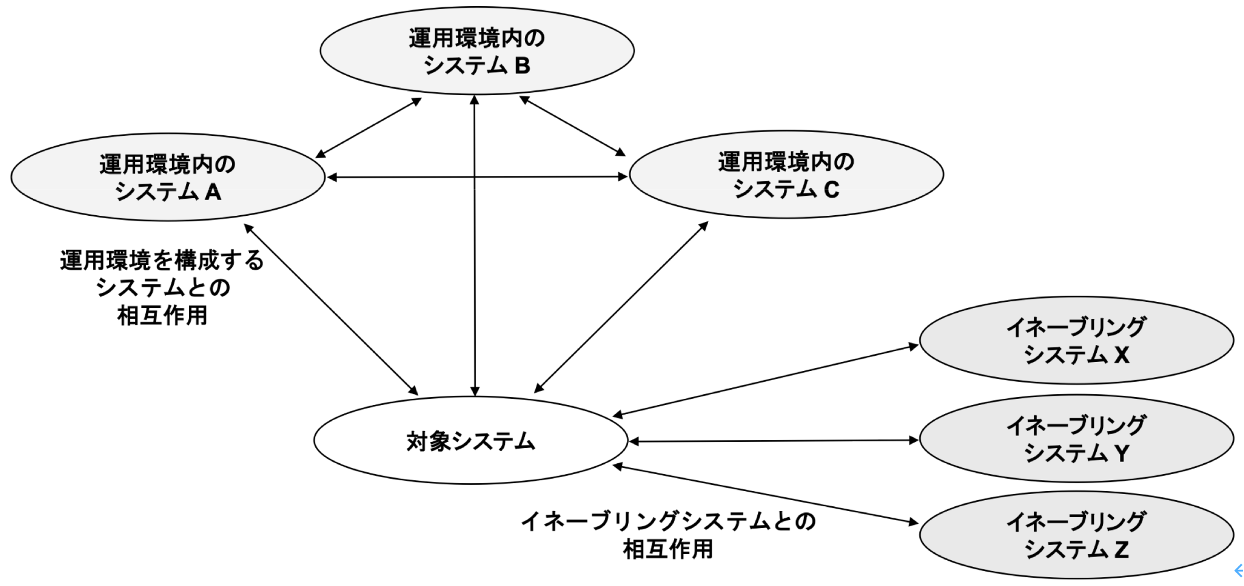
\includegraphics[width=100mm,bb=0 0 622 293]{safety_assurance_contents/ch4images/fig1.png}
    \caption{イネーブリングシステム}
    \label{figure:ch4-1}
    \end{center}
\end{figure}

\subsection{システムの開発や運用においてありうる活動の定義}

システムエンジニアリングでは、システム開発に関わる活動を分類し、標準化
したものとしてシステムライフサイクルプロセス(system lifecycle
  processes)が定義されています。ISO/IEC/IEEE 15288:2023による定義を
\ref{figure:ch4-2}に示します。
\begin{figure}
    \begin{center}
    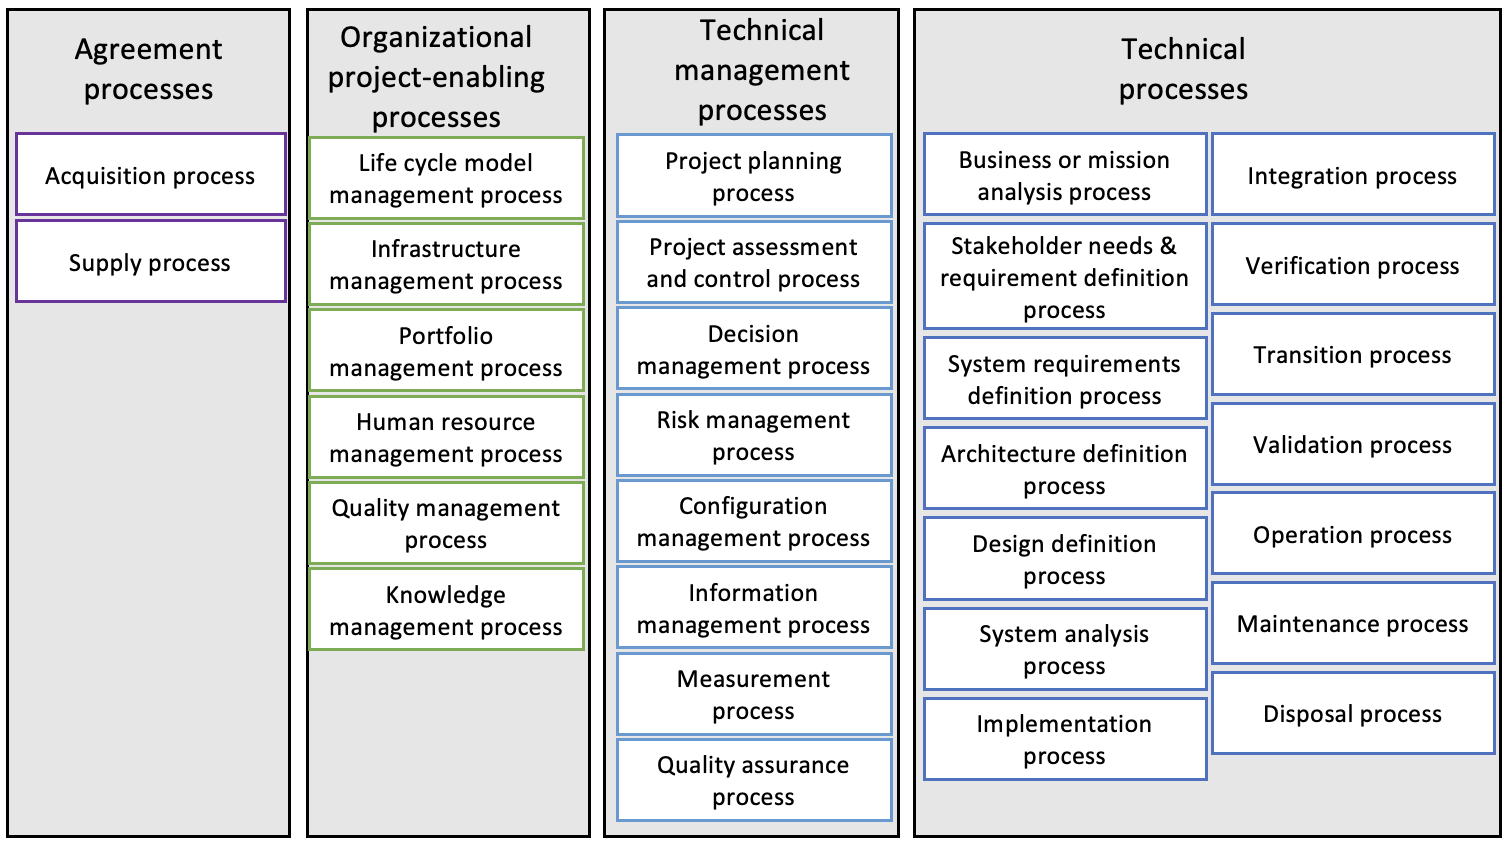
\includegraphics[width=100mm,bb=0 0 756 424]{safety_assurance_contents/ch4images/fig2.png}
    \caption{システムライフサイクルプロセス}
    \label{figure:ch4-2}
    \end{center}
\end{figure}

システムのライフサイクルを通じて、システムに係わる活動は、ここに挙げら
れているどれかのプロセスに相当すると考えることができます。注意点として
は、これらのプロセスは順序を定義しているものではないということです。プ
ロセスの順序は、ライフサイクルモデル(lifecycle model)として定義され、
異なる概念として理解されます。

これらのライフサイクルプロセスは以下の4つに分類されます:

\begin{itemize}
    \item 合意プロセス(agreement processes)
    \item 組織のプロジェクトイネーブリングプロセス(organizational project-enabling processes)
    \item テクニカルマネジメントプロセス(technical management processes)
    \item テクニカルプロセス群(technical processes)
\end{itemize}

これらのプロセス群には、システムの直接的な開発活動だけでなく、それを支援
する活動も含んでいます。例えば、テクニカルプロセスには、技術者には馴染
み深い設計定義プロセス(design process)や実装プロセス
(implementation)、運用プロセス(operational process)などが含まれて
おり、イメージしやすいと思われます。一方で、システムズエンジニアリング
で提供されるライフサイクルプロセスはそれらだけではありません。プロジェ
クトを計画するプロジェクト計画プロセス(project planning process)や、
人員の確保や配置などの活動を含む人的リソースマネジメントプロセス
(human resource management process)、さらには、契約に係わる活動であ
る取得プロセス(acquisition process)や供給プロセス(supply process)
などまで含まれています。これは、これまでのシステムズエンジニアリングの
知見において、システムを開発する際には、直接的な開発活動だけでなく、そ
れを支える活動も含めて考える必要があることを表しています。

\subsection{システムを記述するために必要な観点の提供}

システムを開発したり、運用したりするためには、対象システムを記述する必
要があります。その記述方法についてもシステムズエンジニアリングは知見を
与えてくれます。

一般に、大規模なシステムは、一つの設計図だけではその全貌を現すことはで
きません。そのため、例えば、詳細な記述の前に、その概要だけを記した文章
や設計図なども作成します。従来からそのような記述を「アーキテクチャ設計」
や概要設計と呼んでいました。ただし、概要を把握するにしても、目的やそれ
を読む関係者に応じて複数の記述を作成することが一般的です。それではどの
ような記述が「アーキテクチャ」とよべるのでしょうか。アーキテクチャの記
述は一般にはシステムの抽象的なものです。ただし、抽象的であればアーキテ
クチャというわけでもありません。なぜ抽象化された記述なのに、それが利用
されるかと言えば、システムに関する何らかの関心事を表していたり、懸念事
項を確認できたりすることが期待されるからです。また、ここでの「関心事」
や「懸念事項」は、それを持つ主体が想定されます。システムに関して関心や
懸念を持つ主体を広くステークホルダー(stakeholder, 利害関係者)と呼び
ます。ここで、なんらかのしステークホルダーのなんらかの関心事(concern)
を表現したものをアーキテクチャビュー(architecture view)と呼びます。
アーキテクチャ記述(architecture description)は、このビューの集まりで
あると定義されます。

さらに、ステークホルダーとその関心事は、典型的なものはパターン化してお
くと便利であり、かつ、その記述方法は、おのずと適切に表現できる記法がき
まってくることが多いです。このような、ステークホルダーとその関心事、そ
の表現方法をまとめたものをアーキテクチャビューポイント(architecture
  viewpoint)と呼ばれます。アーキテクチャビューとアーキテクチャビュー
ポイントのイメージは次のような図で説明されることがありま
す~(\ref{figure:ch4-3})。

\begin{figure}
    \begin{center}
    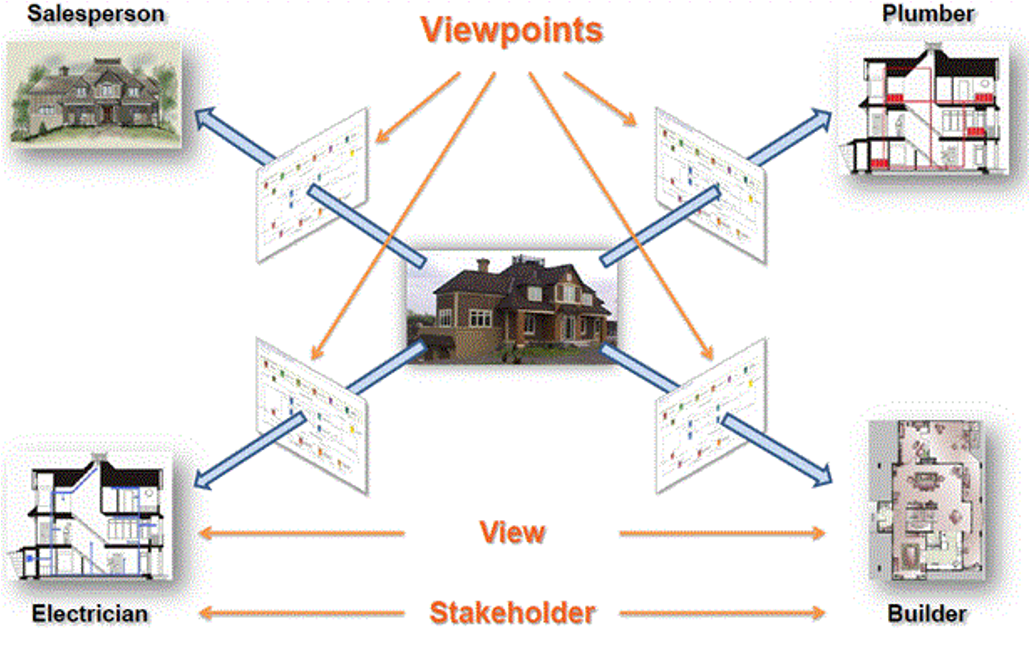
\includegraphics[width=100mm,bb=0 0 515 323]{safety_assurance_contents/ch4images/fig3.png}
    \caption{アーキテクチャビュー及びアーキテクチャビューポイントのイメージ}
    \label{figure:ch4-3}
    \end{center}
\end{figure}

原理的にはシステム毎にステークホルダーやその関心事は異なるため、アーキ
テクチャビューポイントはシステム開発のプロジェクト毎に構築しなければな
らないように見えますが、一般的に多くのプロジェクトで使用可能なアーキテ
クチャビューポイントの集まりもいくつか提供されています。ここでは、その
中からアーキテクチャビューポイントの具体例を紹介します。

\begin{itemize}
\item オペレーショナルビューポイント
  \begin{itemize}
\item ステークホルダー $\colon$ ビジネスアーキテクト、経営層
\item 関心事 $\colon$ 対象の論理的なアーキテクチャを明らかにする。
  \end{itemize}
\end{itemize}
ここで提供されている「オペレーショナルビューポイント」のステークホルダー
は、経営層やビジネスアーキテクトと呼ばれる人たちです。関心事の「論理的
  なアーキテクチャ」とは、実現方法や実装方法に依存しない論理的な構造や
振る舞いを記述するアーキテクチャを指します。もし対象システムのステーク
ホルダーに経営層やビジネスアーキテクト相当の人たちが係わっている場合、
まずはこのような一般的に提供されているビューポイントから、それらステー
クホルダーに関係しそうなビューポイントの記述を参考に、必要なビューポイ
ントを定義することができます。

\section{モデルベースドシステムズエンジニアリング(MBSE)}

\subsection{MBSEの概念}

モデルベースドシステムズエンジニアリング(model-based systems
  engineering, MBSE)は、モデルを活用したシステムズエンジニアリングの
アプローチです。ここでいうモデルとは、ある対象に対して、その対象の特徴
を理解したり予測したりするために用いられる抽象的な表現を指します。例え
ば、次の図はモデルの例です。
\begin{figure}
    \begin{center}
    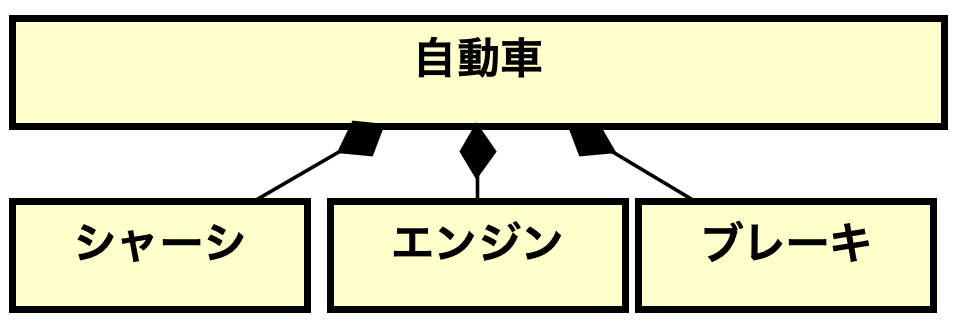
\includegraphics[width=60mm]{safety_assurance_contents/ch4images/fig4.png}
    \caption{モデルの例}
    \label{figure:ch4-4}
    \end{center}
\end{figure}
ここでは図の詳しい表記法の説明はしませんが、自動車はシャーシ、エンジン、
ブレーキという構成要素からなっていることを表現しています。とても単純で
すが、これによって例えば、自動車を開発するにあたって、「シャーシ」「エ
  ンジン」「ブレーキ」を開発する必要があることを伝えるためには、これで
十分です。一方で、次の図もモデルの例です。
\begin{figure}
    \begin{center}
    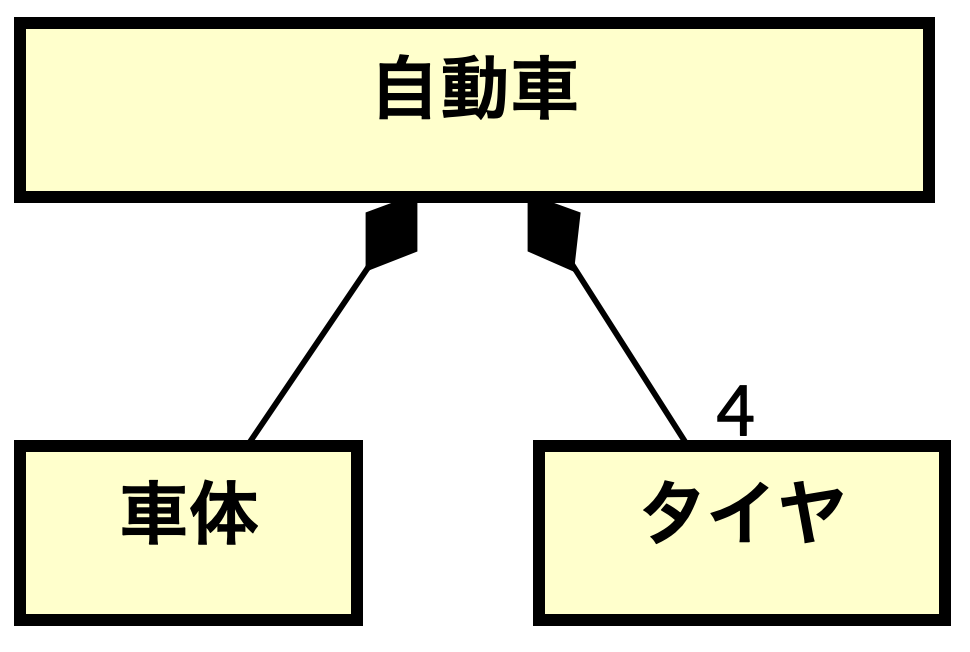
\includegraphics[width=40mm]{safety_assurance_contents/ch4images/fig5.png}
    \caption{モデルの別の例}
    \label{figure:ch4-5}
    \end{center}
\end{figure}
このモデルは、モデルは車体と四つのタイヤから構成されていると主張してい
ます。この図は自動車は、自動車やオートバイと比べて、四輪のタイヤからな
ることが特徴であることを表現しています。同じ自動車の構成要素を表すモデ
ルでも、二通りのモデルを定義できました。これらはどちらが正しいというも
のではなく、「その対象の特徴を理解したり予測したりする」ことに依存して
そのモデルが適切か否かが議論されるものです。

\subsection{SysML(Systems Modeling Language)}

SysMLは、システムズエンジニアリングのための代表的なモデリング言語です。
前節の\ref{figure:ch4-4}や\ref{figure:ch4-5}はSysMLの記述例です。
実際にはいくつかの図的表現の集合として定義されています。それらは次の四
つに大きく分類されます。
\begin{enumerate}
    \item 構造
    \item 振る舞い
    \item パラメータ
    \item 要求
\end{enumerate}
ここにもシステムズエンジニアリングの知見が反映されています。システムの
抽象的な表現には無数の可能性がありますが、システムズエンジニアリングの
目的を達成するためには、上記四つの分類で概ね必要十分であることを意味し
ています。

構造のモデルでは、システムを構成する要素とその関係を表現します。例えば、
自動車をシステムとみなした場合、エンジン、シャーシ、車体などの構成要素
とそれらの関係を表現します。

振る舞いのモデルでは、システムの動作や状態遷移を表現します。自動車の例
でいえば、エンジンの始動から停止までの状態遷移などを表現します。

パラメータモデルでは、システムの性能や特性を決定する要因間の関係を表現
します。例えば、自動車の場合、エンジン出力と最高速度の関係、車体重量と
燃費の関係などを表現します。

要求のモデルでは、システムが満たすべき条件や制約を表現します。例えば、
自動車の場合、消費者からの要望や潜在的なニーズに加え、安全性基準、燃費
基準、排出ガス規制などが要求のモデルとして記述されます。

一見、これら四つに含まれていないように見えるシステムの側面について検討
してみましょう。

例えば、重要な要因であることには疑いがないコストはどうでしょうか。直接
コストのモデルとは書いていませんが、例えば、パラメータのモデルの一つの
パラメータになります。また、パラメータの一つであるコストの評価のために
は、コンポーネント毎に調達コストが決まっていれば、それらコンポーネント
の構成を表す構造のモデルが必要になります。また、どの程度のコストまで許
容できるかは要求に係わる要因になります。

\subsubsection*{練習問題}
例えば、あるシステムではユーザビリティ(使いやすさ)が重要な要因である
ことが分かりました。ユーザビリティに関して、構造、振る舞い、パラメータ、
要求の四つの側面から議論せよ。

\section{トレードオフ分析}

\subsection{トレードオフ分析の概要}

トレードオフ分析は、システムの異なる特性や性能間の関係を評価し、最適な
解決策を見出すプロセスです。多くの場合、ある特性を向上させると他の特性
が低下するという関係があり、これらのバランスを取ることが重要です。

\subsection{記述型モデルと分析型モデルの連携}

トレードオフ分析を効果的に行うためには、記述型モデルと分析型モデルの連
携が重要です。

\begin{itemize}
    \item 記述型モデル:SysMLなどを用いて、システムの構造、振る舞い、
      要求などを記述します。ステークホルダー間のコミュニケーションや合
      意形成に役立ちます。
    \item 分析型モデル:MATLAB/Simulinkなどのツールを用いて、システム
      の性能や動作をシミュレーションします。定量的な評価や予測に役立ち
      ます。
\end{itemize}

\subsection{トレードオフ分析の手順}

以下の手順でトレードオフ分析を行います:

\begin{enumerate}
    \item ソリューション案の検討と妥当性確認
    \item 分析ケースの検討と妥当性確認
    \item パラメータ項目/値の検討と妥当性確認
    \item シミュレーションなどによる分析の実施
    \item 分析結果の評価と意思決定
\end{enumerate}

\section{事例: 巨大ショッピングセンターの駐車場}

ここでは、巨大ショッピングセンターの駐車場を例にシステムズエンジニアリ
ングの実践を見ていきます。\ref{figure:ch4-6}に巨大ショッピングセンター
のイメージを示します。
\begin{figure}
    \begin{center}
    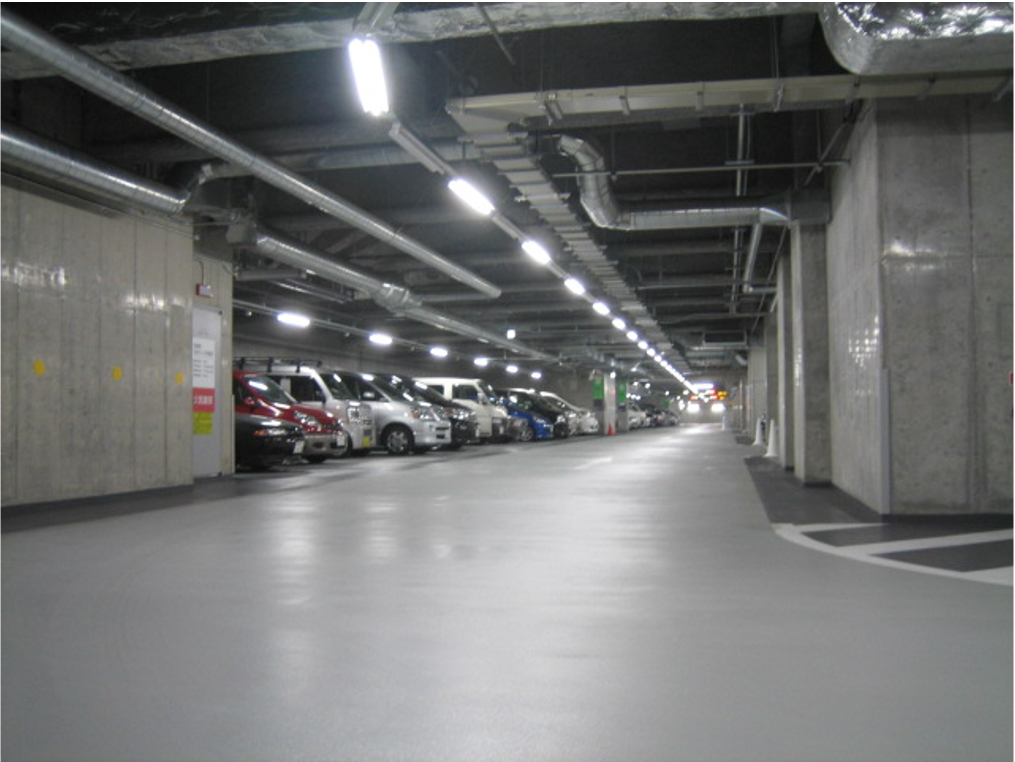
\includegraphics[width=70mm]{safety_assurance_contents/ch4images/fig6.png}
    \caption{巨大ショッピングセンターの駐車場のイメージ}
    \label{figure:ch4-6}
    \end{center}
\end{figure}
ある巨大ショッピングセンターで以下のような課題が問題に
なっていると想定します。
\begin{itemize}
\item
  駐車した場所から目的地である売り場まで遠い
\item
  自分の駐車した場所を忘れる
\item
  人のクルマにぶつける/ぶつけられる
\item
  子供を連れていると危ない
\end{itemize}
また、本事例においては、単独のシステム開発では無く、複数のシステムの連
携についても扱いたいため、以下のような想定を置きます。
\begin{itemize}
\item
  ある程度自動運転車が普及してきている世の中を想定
\end{itemize}
\subsection{本事例の流れ}
それでははじめに、本事例におけるシステムズエンジニアリング活動の流れを
示します。ここでは特に、システムズエンジニアリングにおけるアーキテクチャ
の記述に絞って例を示します。アーキテクチャのライフサイクルは、国際標準
規格であるISO/IEC/IEEE42020\lbrack ISO/IEC/IEEE42020\rbrack や統一アー
キテクチャフレームワークのエンタープライズアーキテクチャガイド\lbrack
Enterprise Architecture Guide\rbrack、TOGAF などに詳しく書いてあります。
ここではそれらを参考に簡単なアーキテクチャライフサイクルを定義します。

\begin{figure}
    \begin{center}
    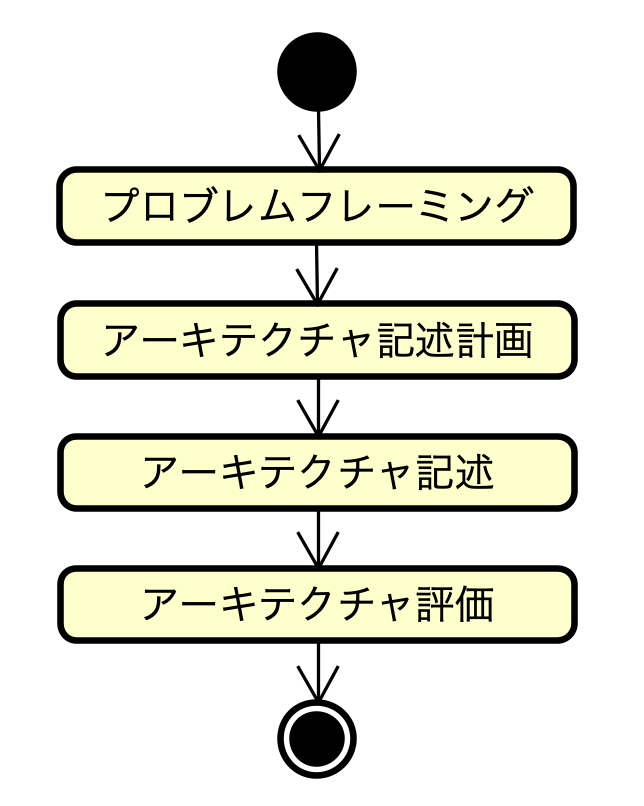
\includegraphics[width=50mm]{safety_assurance_contents/ch4images/fig8.png}
    \caption{事例におけるアーキテクチャライフサイクル}
    \label{figure:ch4-6}
    \end{center}
\end{figure}
まずはじめに、アーキテクチャで記述すべき課題を明示化し、特徴付けするプ
ロブレムフレーミングを実施します。ここでは特にモデルは使わずに、この後
のアーキテクチャ活動の対象や、アーキテクチャによって明らかにしたいこと
などに関する共有の理解を得ることを目指します。次のアーキテクチャ記述計
画では、設定した課題に対して、どのようなアーキテクチャを記述するのかを
決めます。例えば、使用するビューポイントなどを決めていきます。あとは、
実際にアーキテクチャを記述し、評価します。
\subsubsection{プロブレムフレーミング}
ここでは、アーキテクチャを記述することによって解決したい課題を簡潔に表
現したプロブレムステートメント及びアーキテクチャを記述する上で前提とする
仮定を定義します。

プロブレムステートメントは例えば次のように書けます。

\begin{screen}
プロブレムステートメント: 以下の課題を解決する次期駐車場システムのアー
キテクチャを明らかにする。
\begin{itemize}
\item
  駐車した場所から目的地である売り場まで遠い
\item
  自分の駐車した場所を忘れる
\end{itemize}
\end{screen}

仮定の記述例を示します。
\begin{screen}
  仮定: ある程度自動運転車が普及してきている世の中を想定。ただし、駐車
  場内での自動運転には対応していない。
\end{screen}
\subsubsection{アーキテクチャ記述計画}
アーキテクチャ記述に使用するビューポイントの定義などを実施します。ビュー
ポイントの定義のためには、ステークホルダーを識別し、それぞれの関心事を
記述し、関心事が表現できるモデルを決定するという手順になります。ここで
は、UAFをベースに、以下のビューポイントが得られたと想定します。
\begin{itemize}
\item
  \textbf{戦略ビューポイント} 経営層などが関心の
  ある意思決定に必要な情報を表現します。モデルは以下の種類を使用します。
  \begin{itemize}
  \item
    動機のモデル: 対象の背景となっている課題を分析したり、共通認識を得
    るために使用します。
  \item
    能力のモデル: 最上位レベルの要求の表現として、次期駐車場システム全
    体がもつべき能力を表現します。
  \item
    効果のモデル: 能力が達成した際に得られる効果を表現します。
  \item
    測定量のモデル: 効果に対する指標を表現するための測定量を定義します。
  \end{itemize}
\item
  \textbf{運用ビューポイント} 論理的なアーキテ
  クチャを定義するために使用します。モデルは以下の種類を使用します。
  \begin{itemize}
  \item
    論理的な活動のモデル: 能力を実現するために必要な活動を定義します。
  \item
    トレーサビリティのモデル: 能力と論理的な活動とのトレーサビリティを
    定義します。
  \end{itemize}
\item
  \textbf{リソース及び人員ビューポイント} 具体的なシステムや人員体制な
  どのアーキテクチャを表現します。モデルは以下の種類を使用します。
  \begin{itemize}
  \item
    リソース及び人員の語彙のモデル: 能力実現に必要なリソース及び人員を
    列挙し、自然言語で定義する。
  \end{itemize}
\end{itemize}
ベースとしたUAFのビューポイントはそれぞれStrategic Viewpoint、Operational Viewpoint、
Resource Viewpointとなります。
\subsubsection{アーキテクチャ記述}
それでは、具体的にアーキテクチャを記述して行きます。
まずは、戦略ビューポイントの動機のモデルを記述例を示します。
\begin{figure}
    \begin{center}
    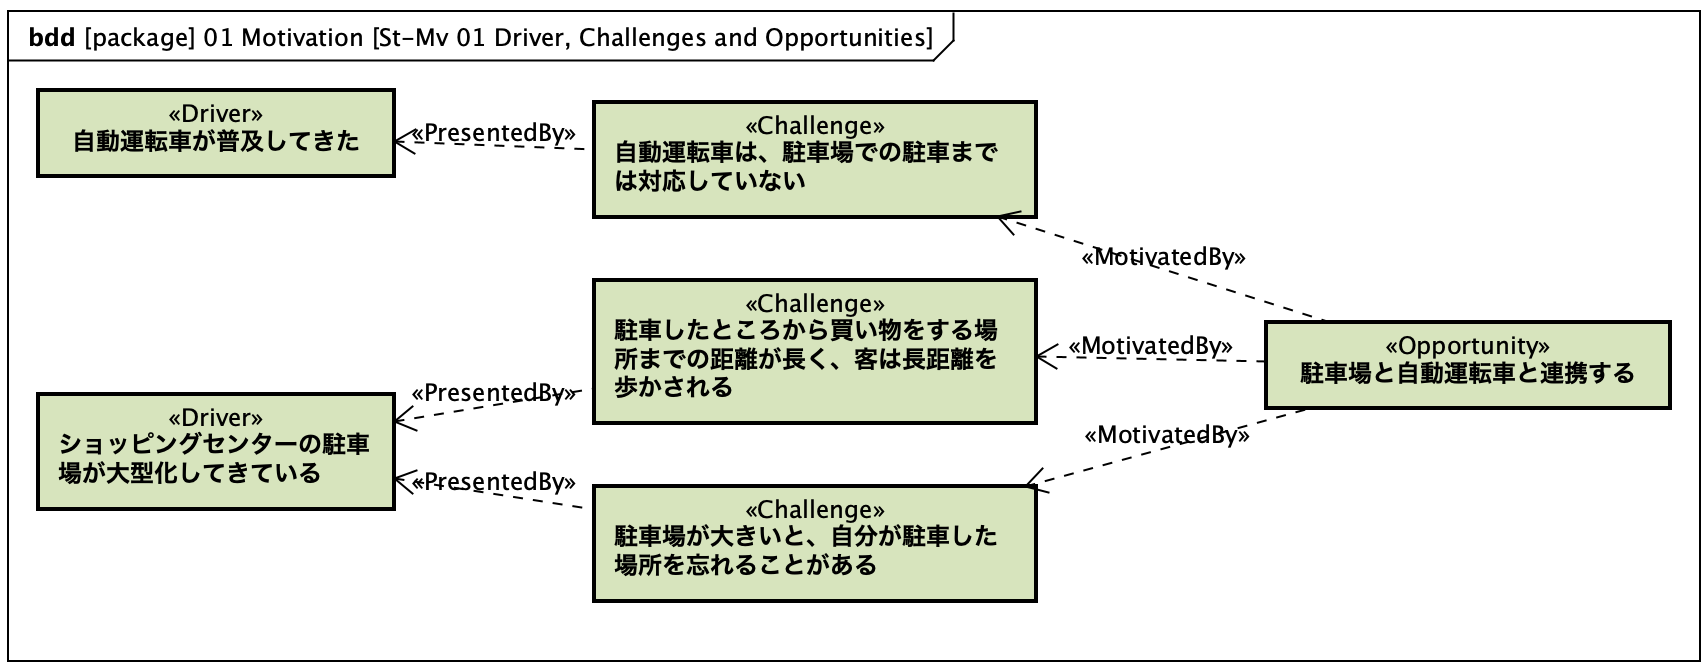
\includegraphics[width=50mm]{safety_assurance_contents/ch4images/fig9.png}
    \caption{事例:戦略ビューポイントの動機のモデル}
    \label{figure:ch4-7}
    \end{center}
\end{figure}
\begin{itemize}
\item ショッピングセンター近くの巨大な立体駐車場を対象
\item 利用者は駐車場入口でクルマから降り、アプリで自動駐車を指示
\item 車両は自律的に空きスペースまで移動し駐車
\item 引き取り時も、アプリで指示後に車両が自動で出庫
\end{itemize}
\subsection{ステークホルダーの識別}


\subsection{能力の定義と評価指標}

システムに求められる能力とその評価指標を定義します:

\begin{itemize}
    \item 能力:自動駐車機能
    \item 評価指標:
    \begin{itemize}
        \item 平均入庫時間
        \item 平均出庫時間
        \item 平均待ち時間
        \item 安全度レベル
        \item 利用者ストレスポイント
    \end{itemize}
\end{itemize}

\subsection{リソースアーキテクチャの検討}

システムを構成するリソースとその構造を検討します。主要なコンポーネントには以下が含まれます:

\begin{itemize}
    \item 自動運転機能付き車両
    \item 駐車場管理システム
    \item 空きスペース確認システム(固定カメラまたはドローン)
    \item ユーザーインターフェース(スマートフォンアプリ)
\end{itemize}

\subsection{分析ケースの定義}

システムの評価のための分析ケースを定義します。考慮すべき要素には以下が含まれます:

\begin{itemize}
    \item 自動運転車普及率(例:20%、80%)
    \item 来客状況(閑散期、繁忙期)
    \item 駐車場の構造と容量
    \item 周辺交通状況
\end{itemize}

\subsection{シミュレーションと分析}

定義した分析ケースに基づき、MATLAB/Simulinkなどのツールを用いてシミュレーションを行います。また、STAMP/STPAなどの手法を用いて安全性分析を実施します。

\subsection{結果の評価とトレードオフ分析}

シミュレーションと分析の結果を評価し、各ソリューション案のトレードオフを検討します。例えば:

\begin{itemize}
    \item 固定カメラ方式:初期コストは低いが、スケーラビリティに課題
    \item ドローン方式:柔軟性が高いが、安全管理に追加コストが必要
\end{itemize}

これらの結果を総合的に判断し、最適なソリューションを選択します。

\section{まとめ}

システムエンジニアリングは、複雑なシステムの開発と管理を体系的に行うための重要なアプローチです。MBSEやSysMLの活用、そしてトレードオフ分析の実施により、以下のような利点が得られます:

\begin{itemize}
    \item システムの全体像と詳細の両方を把握できる
    \item ステークホルダー間のコミュニケーションが促進される
    \item 定量的な評価に基づく意思決定が可能になる
    \item システムの品質、信頼性、安全性の向上につながる
\end{itemize}

今後のシステム開発者は、これらの手法と考え方を効果的に活用し、より良いシステムを設計・開発することが求められます。
\subsection{参考文献}
\begin{itemize}
\item
  \lbrack JIS X 0170\rbrack\ \ JIS X 0170: 2020 システムライフサイクルプロセス (ISO/IEC/IEEE15288:2015)
\item
  \lbrack ISO/IEC/IEEE42020\rbrack\ \ ISO/IEC/IEEE42020:2019 Architecture Processes
\item
  \lbrack UAF \rbrack\ \ Unified Architecture Framework(UAF) Domain Metamodel, Version 1.2, OMG, December 2021.
\item
  \lbrack Enterprise Architecture Guide\rbrack\ \ Enterprise Architecture Guide for UAF (Informatice), Appendix C, Version 1.2, OMG, July 2022.
\end{itemize}
